\documentclass [12pt, a4paper, twoside, titlepage] {article}

\usepackage{booktabs}% http://ctan.org/pkg/booktabs
\usepackage{graphicx}% http://ctan.org/pkg/graphicx
\usepackage{tabularx}
\usepackage{varwidth}% http://ctan.org/pkg/varwidth
\usepackage[T1]{fontenc}
\usepackage{lmodern}
\usepackage[top=2.5cm, bottom=2.5cm, left=2.5cm, right=2.5cm, footskip=2cm]{geometry}
\usepackage{lastpage}

\usepackage{fullpage}
\usepackage{moreverb}
\usepackage{alltt}
\usepackage{boxedminipage}
\usepackage{fancyhdr}
\usepackage{lastpage}
\usepackage{hyperref}
\usepackage{listings}
\usepackage{placeins}

\usepackage{pdfpages}

\newcommand{\turn}[3][10em]{% \turn[<width>]{<angle>}{<stuff>}
  \rlap{\rotatebox{#2}{\begin{varwidth}[t]{#1}\bfseries#3\end{varwidth}}}%
}


\newcommand*{\defined}{\textbf}

\newcommand{\documentVersion}{V 1.0 }

\newcommand{\documentName}{Test Report - ArrayStack }

\pagestyle{fancy}
\lfoot{\documentName}
\cfoot{\thepage\ of \pageref{LastPage} }
\rfoot{\documentVersion \date{\today}}
\headheight 20pt
\headsep 10pt

\raggedbottom

\begin{document}


\title{\documentName}

\author{Tim Pizey
\\Oxford University
\\\tt{Tim.Pizey@gmail.com}
\\
\\Page count \pageref{LastPage}
}
\date{\today}

\maketitle


\addtocontents{toc}{\protect\newpage}
\newpage
\lfoot{\documentName}
\setcounter{section}{0}
\part{Test Report}
\section{Test Environment}
The tests should be run on all target hardware and operating systems, given below are the versions actually run on due to limitations of available testing setup :\\
\begin{tabular}{llll}
\hline
\textbf{Processor} & \bf{OS} & \bf{Memory}& \bf{Java\texttrademark Version}\\
\hline
  Intel Core 2 Duo      & OSX 10.6.8 & 4 GB & HotSpot$(TM)$ 64-Bit version 1.6.0\_37 \\
  Intel i7      & Ubuntu 12.0.4 & 8 GB &  OpenJDK 64-Bit version 1.7.0\_09 \\
\hline
\end{tabular}
Current versions of Java\texttrademark are able to simulate earlier versions and so the tests have been 
run with simulated Java\texttrademark versions 1.3, 1.4, 1.5, 1.6 and 1.7. 

The tests were run with JUnit version 3.8.1.

\section{Additional Test Machinery}
The defects in the SUT prevent the full tests being run successfully, as \textbf{JUnit} fails at the first failing assertion in a test. 
These defects would normally be fixed, to enable the next defect to be detected.
For the purposes of this example a new class \texttt{FixedStackArray} is supplied on which all the tests run to completion, 
in a real world development the fixes would  be applied directly to the SUT. 

Some machinery is introduced to enable the tests to be run on both 
classes, exposing another design smell: the method \texttt{atPosition(int p)} is not specified in the 
interface \texttt{jdslcomp.simple.api.Stack} so we cannot test cleanly to the \texttt{Stack} interface.


\section{Test Design} 

The tests are designed using a combination of categorisation, analysis and inspection .
\subsection{Method Categories}

\begin{table}[!htbp]
\begin{tabular}{|lll|}
\hline
\bf{Creation} & \bf{Transforming} & \bf{Non-transforming} \\ 
\hline
Default constructor & push & size \\
Sized constructor & pop & isEmpty \\
&& top \\
&& atPosition\\
&& toString \\
\hline
\end{tabular}
\caption{Method Categories}
\label{tab:methodTypes}
\end{table}

\subsection{Analysis of Argument Types}
The semantic type of the \texttt{size} argument to the constructor is  \textbf{Positive Integer Greater Than Zero} which ranges from \texttt{1} to \texttt{Infinity} however it is implemented using the Java\texttrademark primitive \texttt{int} which ranges from \texttt{Integer.MIN\_VALUE} to \texttt{Integer.MAX\_VALUE} ie it includes negative integers and zero and it has an upper bound. 
We need to test that the SUT correctly handles all cases where the range of the implementation does not coincide with the range of the semantic type. 

Similarly the \texttt{position} argument has the same semantic type,   \textbf{positive Integer Greater Than Zero}, but is implemented as  \texttt{int}  so the same checks need to be made. In addition we know that the SUT is implemented using a java  \texttt{Object} array 
which uses a zero based index so we need to test for a mis-match between the \texttt{position} in the abstract \texttt{Stack} and the concrete \texttt{index} of the array.


\subsection{State Transition Analysis}

The  state model in Figure \ref{stackStates} shows the effect on the System Under Test (SUT) 
of the two state transforming methods \texttt{push} and \texttt{pop}, the creation and 
non-transforming methods are excluded for clarity.
\begin{figure}[H]
\setlength\fboxsep{0pt}
\setlength\fboxrule{0.5pt}
\fbox{
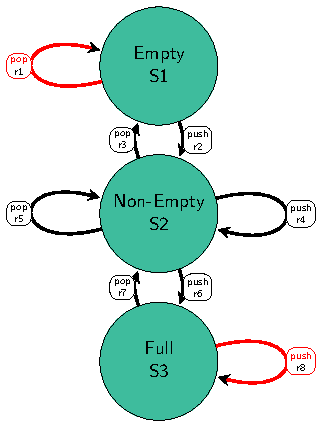
\includegraphics[width=\textwidth]{stackStates.pdf}}
\caption{Stack States, exception transitions are coloured in red}
\label{stackStates}
\end{figure}

\begin{table}[!htbp]
\begin{tabular}{rlrlrrl}
\textbf{Edge} & \textbf{Operation} & \textbf{Before} & \textbf{After} & \textbf{Transition} & \textbf{Return} & \textbf{testName} \\ 
\hline\\
r1 & pop & S1 & S1 &  no & Exception & testPopFromEmpty \\

r2 & push & S1 & S2 & yes & void & testPushToEmpty\\

r3 & pop & S2 & S1 & yes & value & testPopEmptying\\

r4 & push & S2 & S2 & no & void & testPushCentral\\

r5 & pop & S2 & S2 & no & value & testPopCentral\\

r6 & push & S2 & S3 & yes & void & testPushFilling\\

r7 & pop & S3 & S2 & yes & value & testPopFromFull\\

r8 & push & S3 & S3 & no & Exception & testPushToFull\\  
\hline
\end{tabular}
\caption{State Table}
\label{tab:stateTable}
\end{table}
\FloatBarrier

\subsection{Thread Safety Analysis} 

To use the \texttt{ArrayStack} in a multi-threaded setting it is necessary to \texttt{synchronize} on the stack. 
It is not sufficient to \texttt{synchronize} the \texttt{push} and \texttt{pop} methods as shown in \texttt{testUnsafeThreadedAccess()}.


\subsection{Memory Leak Analysis}
findbugs does not report any anti-patterns.

\subsection{Failure Modes Analysis}

Two modes of failure have been highlighted: memory exhaustion, where the initial size of the stack is greater than the available memory, exposed by \texttt{testMaxConstructor()}, the correct exception is thrown. 

The second failure, highlighted in \texttt{testUnsafeThreadedAccess()}, arises from misuse: 
failure to \texttt{synchronize} upon the stack object in a multithreaded environment 
will lead to thread clashes and unexpected results. This is not a defect and cannot be changed but should be documented.

\subsection{Security Analysis}

No security issues are considered at this level.

\section{Tests}
\lstset{language=Java, frame=tlrb, rulesepcolor=\color{blue}}
\lstset{ caption=Tests, label=tests}
\lstinputlisting{/Users/timp/git/arraystack/src/test/java/ArrayStack/ArrayStackSpec.java}

\lstset{ caption=ArrayStackTest, label=ArrayStackTest}
\lstinputlisting{/Users/timp/git/arraystack/src/test/java/ArrayStack/ArrayStackTest.java}
\lstset{ caption=FixedArrayStackTest, label=FixedArrayStackTest}
\lstinputlisting{/Users/timp/git/arraystack/src/test/java/ArrayStack/FixedArrayStackTest.java}

\section{Results}
\subsection{Jenkins Results}
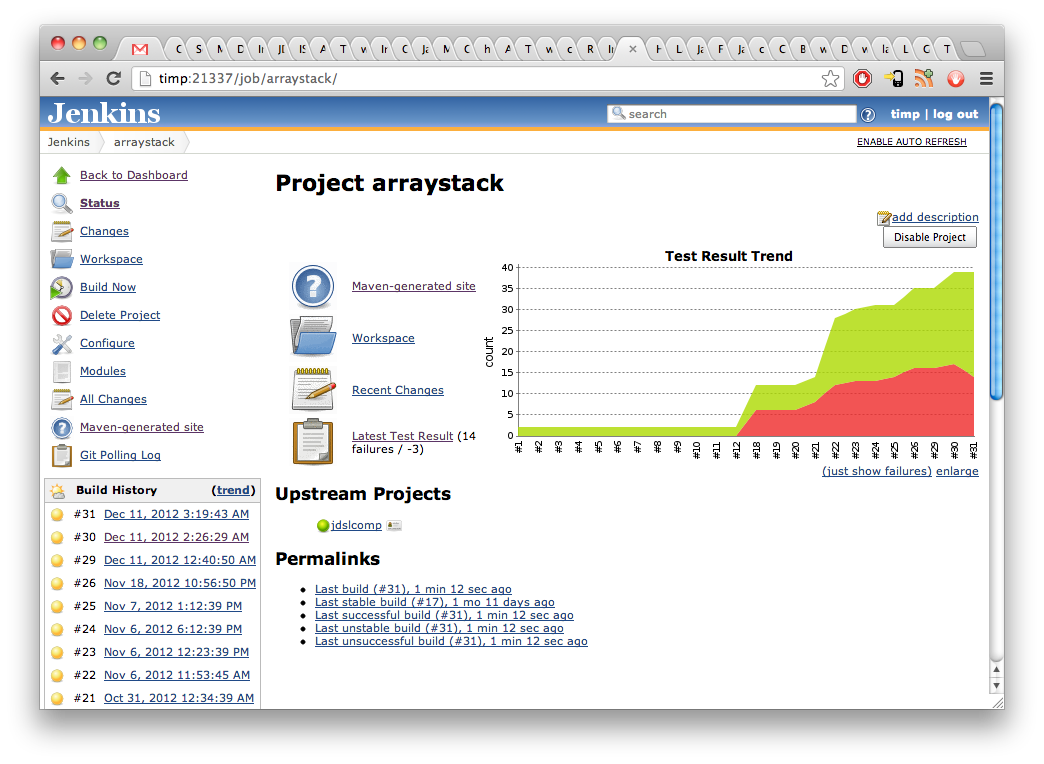
\includegraphics[width=18cm]{JenkinsResults.png}
\subsection{Static Analysis Reports}
\subsubsection{Cobertura}
Cobertura shows an uncovered line in \texttt{push(Object o)} caused by defect AS02.\\

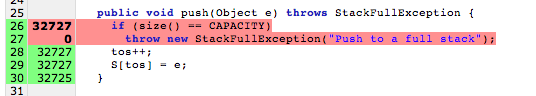
\includegraphics{cobertura.png}



\subsubsection{Findbugs}
Findbugs discovers two performance issues which can be safely ignored.\\
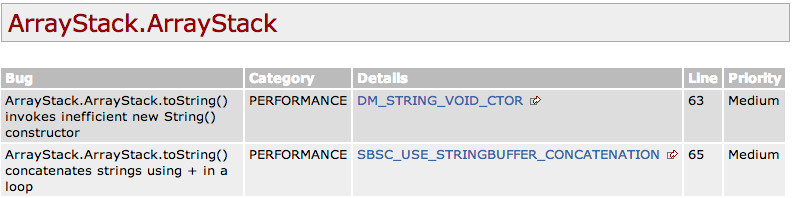
\includegraphics[width=18cm]{findbugs.png}

\subsubsection{Checkstyle}
Checkstyle finds 40 style issues, from the trivial "File does not end with a newline", through design pattern checks  
"Method 'isEmpty' is not designed for extension - needs to be abstract, final or empty.". 

Checkstyle needs to be configured carefully but can be useful, each issue is worth considering, 
even if to positively configure Checkstyle not to perform that check.

\subsubsection{PMD}
PMD found no issues.

\subsubsection{CPD}
Not surprisingly picked up the similarities between ArrayStack.java and FixedArayStack.java.

\subsubsection{JDepend}
JDepend produces a summary of its quality metrics, and an explanation of the code quality model it uses.\\

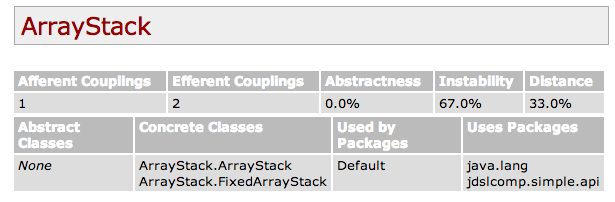
\includegraphics[width=16cm]{jdepend.png}


\subsection{Surefire Results}

\begin{tabularx}{\textwidth}{lllr}
\hline
 & & \textbf{ArrayStackTest} & \\
\hline
Test & Status & Reason & Time \\
\hline 
testNegativeSizeConstructor  & Failed & Threw  NegativeArraySizeException &  0.004 \\
testZeroSizedConstructor  & Failed &  Should have bombed &  0 \\
testOneConstructor & Failed & Attempt to go beyond top of stack &  0.004 \\
testThreeConstructor  & Failed &  Attempt to go beyond top of stack & 0 \\
testCapacityConstructor  & Failed &  Attempt to go beyond top of stack & 0 \\
testMaxConstructor  & Passed &  &  0 \\
testDefaultConstructor  &  Failed & Attempt to go beyond top of stack & 0 \\
testPushNull& Passed & & 0\\
testBadPosition  &  Failed & ArrayIndexOutOfBounds -2 & 0\\
testPopFromEmpty & Passed & & 0\\
testPushToEmpty  &  Failed & expected:<1> but was:<> & 0\\
testPopEmptying& Passed & & 0\\
testPushCentral  &  Failed & expected:<1 2> but was:<2 > & 0.001\\
testPopCentral  & Failed & expected:<1> but was:<> & 0\\
testPushFilling  &  Failed & expected:<1> but was:<> & 0 \\
testPopFromFull& Passed & & 0 \\
testPushToFull  &  Failed & ArrayIndexOutOfBounds & 0.001 \\
testThreadedAccess& Passed & & 0.043 \\
testUnsafeThreadedAccess  & Failed &  Failed on iteration 0 & 0.111\\
\hline 
\end{tabularx}

\begin{tabularx}{\textwidth}{lllr}
\hline
 & & \textbf{FixedArrayStackTest} & \\
\hline
Test & Status & Reason & Time \\
\hline 
testNegativeSizeConstructor  & Passed &  &  0\\
testZeroSizedConstructor      & Passed &   &  0 \\
testOneConstructor               & Passed &   &  0 \\
testThreeConstructor  & Passed &  & 0 \\
testCapacityConstructor  & Passed &  & 3.098 \\
testMaxConstructor  & Passed &  &  0.042 \\
testDefaultConstructor  &  Passed &  & 2.849 \\
testPushNull& Passed & & 0\\
testBadPosition  &  Passed &  & 0\\
testPopFromEmpty & Passed & & 0.001\\
testPushToEmpty  &  Passed & & 0\\
testPopEmptying& Passed & & 0\\
testPushCentral  &  Passed &  & 0\\
testPopCentral  & Passed &  & 0\\
testPushFilling  &  Passed &  & 0 \\
testPopFromFull& Passed & & 0 \\
testPushToFull  &  Passed & & 0 \\
testThreadedAccess& Passed & & 0.039 \\
testUnsafeThreadedAccess  & Failed &  Failed on iteration 116 & 0.117\\
\hline 
\end{tabularx}

\subsection{Differences between ArrayStack and FixedArrayStack}



\lstset{caption={AS01, AS02. Capacity bug fix; parameter range check}, label=d1}
\begin{lstlisting}
20,21c20,24
<   public ArrayStack(int cap) {
<     capacity = CAPACITY;
---
>   public FixedArrayStack(int cap) {
>     if (cap < 1)
>       throw new IllegalArgumentException(
>           "A stack must be at least one element big.");
>     capacity = cap;
\end{lstlisting}

\lstset{caption={AS03, AS04. Synchronize push; Capacity bug fix.}, label=as02}
\begin{lstlisting}
25,26c28,29
<   public void push(Object e) throws StackFullException {
<     if (size() == CAPACITY)
---
>   public synchronized void push(Object e) throws StackFullException {
>     if (size() == capacity)
\end{lstlisting}


\lstset{caption={AS05. Synchronize pop}, label=d3}
\begin{lstlisting}
32c35
<   public Object pop() throws StackEmptyException {
---
>   public synchronized Object pop() throws StackEmptyException {
\end{lstlisting}

\lstset{caption={AS06, AS07. Argument checking; tos bug fix}, label=d4}
\begin{lstlisting}
56,57c59,64
<     if (i > tos)
<       throw new StackOutOfScopeException(
>                 "Attempt to go beyond top of stack");
---
>     if (i < 1)
>       throw new IllegalArgumentException(
>           "Stack position must be greater than one.");
>     if (i > (tos + 1))
>       throw new StackOutOfScopeException(
>                 "Attempt to go beyond top of stack ("
>           + i + ">" + (tos + 1) + ")");
\end{lstlisting}

\lstset{caption={AS08. Array index bug fix}, label=d5}
\begin{lstlisting}
64c71
<     for (int i = 1; i < size(); i++)
---
>     for (int i = 0; i < size(); i++)
\end{lstlisting}

\lstset{caption={AS09. Trim toString()}, label=d6}
\begin{lstlisting}
66c73
<     return Sout;
---
>     return Sout.trim();
\end{lstlisting}

\section{Defects}
\begin{table}[!htbp]
\begin{tabularx}{\textwidth}{|r|X|X|X|}
\hline
\textbf{ID} & \textbf{Method} & \textbf{Issue} & \textbf{Recommendation} \\ 
\hline
AS01 & ArrayStack(int cap) & cap not checked for less than zero. & Add parameter check.\\
AS02 & ArrayStack(int cap) & capacity always set to CAPACITY. & Set capacity to cap.\\
AS03 & push(Object e) & Not synchronized. & Add synchronized keyword. \\
AS04 & push(Object e) & CAPACITY instead of capacity. & Change to capacity.\\
AS05 & pop() & Not synchronized. & Add synchronized keyword. \\
AS06 & atPosition(int i) & No parameter lower bounds checking. & Check i greater than zero.\\
AS07 & atPosition(int i) & Position compared to index. & Add one to index to make comparable. \\
AS08 & toString() & First element of array missed. & Start array index from zero. \\
AS09 & toString() & Always ends in a space. & Should be trimmed.\\
AS10 & atPosition(int i) & Method not in interface. & Add to interface or delete method. \\
\hline
\end{tabularx}
\end{table}

\section{Test Assessment}

The tests have revealed some serious defects which must be remedied.
Once remedied, as per FixedArrayStack, the class is fit for purpose.

\subsection{Code Style}
The stylistic flaws identified by Checkstyle should be addressed if the class is to be part of a larger suite.

\subsection{Code Quality}
The threaded tests revealed that the allocation of  a very large stack takes an appreciable length of time. 
There might be performance advantages to allocating 
the stack space when it was needed, rather than allocating the maximum that might be needed,
depending upon whether the maximum stack size is known.

It might be an improvement to create  a \texttt{Position} type and have the bounds checking in 
one place rather than using \texttt{int} for position parameters.

\subsection{Test Improvement}
The test \texttt{testUnsafeThreadedAccess()} should arguably be moved to a separate file where it can 
be easily excluded from running on the Continuous Integration server, as it is a proof that misuse is harmful, 
rather than a failing test.  

\subsection{Documentation Improvement}
The need for synchronization against the stack in multithreaded use should be 
documented in the class javadoc.

The fact that it is possible to create a stack larger than available memory probably does not need to be documented, 
as the same can be said for the creation of any array.
\end{document}
